\documentclass[11pt,oneside]{book}
\usepackage[english, italian]{babel} 
\usepackage{microtype}
\usepackage[utf8]{inputenc}
\usepackage{subfigure}
\usepackage{epsfig}
\usepackage{amsmath, amssymb}
\usepackage[linesnumbered,lined,commentsnumbered,italiano]{algorithm2e}
\usepackage{fancybox}
\usepackage{listings}
\usepackage{url}
\usepackage{graphicx}
\usepackage{todonotes}
\usepackage{moreverb}
\usepackage{lmodern}
\usepackage{multirow}
\usepackage[labelfont=it,textfont={it}]{caption}
\usepackage[final,bookmarks,breaklinks,colorlinks,allcolors=black]{hyperref}
\usepackage{color}
\usepackage[block=ragged,backend=biber,natbib=true]{biblatex} % Use the bibtex backend with the authoryear citation style (which resembles APA)
\addbibresource{bibliography.bib} % The filename of the bibliography
\usepackage[autostyle=true]{csquotes} % Required to generate language-dependent quotes in the bibliography
\usepackage{hyperref}

%%%%%%%%%%%%%%%%%%%%%%%%%%%%
\definecolor{mygreen}{rgb}{0,0.6,0}
\definecolor{mygray}{rgb}{0.5,0.5,0.5}
\definecolor{mymauve}{rgb}{0.58,0,0.82}
\lstset{ %
	backgroundcolor=\color{white},   % choose the background color; you must add \usepackage{color} or \usepackage{xcolor}; should come as last argument
	basicstyle=\footnotesize,        % the size of the fonts that are used for the code
	breakatwhitespace=false,         % sets if automatic breaks should only happen at whitespace
	breaklines=true,                 % sets automatic line breaking
	captionpos=b,                    % sets the caption-position to bottom
	commentstyle=\color{mygreen},    % comment style
	deletekeywords={...},            % if you want to delete keywords from the given language
	escapeinside={\%*}{*)},          % if you want to add LaTeX within your code
	extendedchars=true,              % lets you use non-ASCII characters; for 8-bits encodings only, does not work with UTF-8
	frame=single,
	keepspaces=true,                 % keeps spaces in text, useful for keeping indentation of code (possibly needs columns=flexible)
	keywordstyle=\color{blue},       % keyword style
	morekeywords={*,...},            % if you want to add more keywords to the set
	numbers=left,                    % where to put the line-numbers; possible values are (none, left, right)
	numberstyle=\tiny\color{mygray}, % the style that is used for the line-numbers
	rulecolor=\color{black},         % if not set, the frame-color may be changed on line-breaks within not-black text (e.g. comments (green here))
	showspaces=false,                % show spaces everywhere adding particular underscores; it overrides 'showstringspaces'
	showstringspaces=false,          % underline spaces within strings only
	showtabs=false,                  % show tabs within strings adding particular underscores
	stringstyle=\color{mymauve},     % string literal style
	tabsize=2,	                   % sets default tabsize to 2 spaces
	title=\lstname                   % show the filename of files included with \lstinputlisting; also try caption instead of title
}
%%%%%%%%%%%%%
\definecolor{gray}{rgb}{0.4,0.4,0.4}
\definecolor{darkblue}{rgb}{0.0,0.0,0.6}
\definecolor{cyan}{rgb}{0.0,0.6,0.6}

%%%%%%%%%%%%%%%%%%%%%%%%
\begin{document}
\selectlanguage{italian}

\begin{titlepage}
\begin{center}

\epsfig{file=Figure/logo_standard.jpg,width=2.5truecm}\\[0.2truecm]
{\Large Universit\`a degli Studi di Salerno}\\[0.2truecm]
{\large Dipartimento di Informatica}\\
\hrulefill
\vfill
{\Large GameUp }\\[0.2truecm]
\vfill\vfill
{\Huge System Design Document}
\vfill\vfill


{\bf Studenti} \hfill {\bf Docente}\ \ \\
Francesco Foglia \hfill Prof. Andrea De Lucia\\

\vfill
\hrulefill 

Anno Accademico 2020-2021

\end{center}
\end{titlepage}

\pagenumbering{roman}
\chapter*{Cronologia Revisioni}
\begin{center}
	\begin{tabular}{||c c p{10cm}||} 
	\hline
	Data & Versione & Descrizione \\ [0.5ex] 
	\hline\hline
	09/01/2021 & 1.0 & Analisi iniziale del sistema assieme alla sua scomposizione, la descrizione dei servizi di ciascun sottosistema e alla scelta dei trade-off da rispettare, oltre che al mapping hardware/software e l’analisi delle condizioni limite \\ 
	\hline
	20/01/2021 & 1.1 & Conversione in formato TeX dell'intero documento \\
	\hline
   \end{tabular}
\end{center}

\tableofcontents
\pagestyle{plain}

%%%%%%%%%%%%%%%%%%%%%%%%%%%%
\chapter{Introduzione}
\setcounter{page}{1} 	% devono seguire solo il primo capitolo
\pagenumbering{arabic}	% devono seguire solo il primo capitolo
\input{01SDD_introduzione.tex}

%%%%%%%%%%%%%%%%%%%%%%%%%%%%
\chapter{Architettura del Software Corrente}
Attualmente non esiste un sistema con lo stesso scopo di quello proposto, bensì il sistema proposto trae spunto dalle implementazioni di sistemi simili ma con obiettivi o target diversi. I principali sistemi da cui il sistema corrente prende spunto sono:
\begin{itemize}
	\item \href{https://store.steampowered.com/?l=italian}{Steam}: Uno dei primi e-commerce dedicati ai videogiochi, avente come target il mondo videoludico su computer. Esso offre dei servizi in forma web molto simili al sistema proposto, ma contiene videogiochi unicamente per computer, escludendo completamente altre piattaforme. Anche con un target ristretto, vanta un guadagno di oltre 4 miliardi di dollari annui.
	\item Android Play Store / iOS App Store: I punti di accesso principali sulla gran parte dei dispositivi mobile esistenti. Essi permettono il download di applicazioni compatibili per i dispositivi relativi (Dispositivi Apple per iOS App Store, Dispositivi Android di svariati produttori per Android Play Store), senza un determinato target. Da essi è possibile anche il download di videogiochi mobile, ma non è assolutamente lo scopo principale, non sono offerte funzionalità avanzate di ricerca dedicate a questo tipo di target e non esiste alcun tipo di comunità o forum all’interno di tali piattaforme.
\end{itemize}
Esistono, inoltre, servizi minori per piattaforme attualmente meno usate, come ad esempio Windows Phone, o anche la versione cinese dell’app store, dopo le recenti problematiche tra America e Cina. 

%%%%%%%%%%%%%%%%%%%%%%%%%%%%
\chapter{Architettura del Sistema Proposto}
\section{Panoramica}
Il sistema proposto è una applicazione Web, per garantire la portabilità su quanti più dispositivi possibili nel modo più semplice possibile, così da garantire l’obiettivo di design precedentemente elencato. Lo stile architetturale adattato sarà basato sullo stile architetturale three-tier poiché permette una suddivisione delle componenti essenziali dell’applicazione Web: le pagine HTML mostrate all’utente (con eventuali script) rappresenteranno le nostre interfacce, le richieste mandate dai vari tipi di utenti verranno smistate e gestite dai nostri Controller, i quali manipoleranno i dati nel modo necessario attraverso i nostri Model, i quali agiscono da interfaccia verso le nostre fonti di dati (database e file). I tipi di utenti del nostro sistema saranno di tre tipi: Clienti, Sviluppatori e Amministratori, i quali avranno accesso sia a funzionalità comuni tra di loro, sia a funzionalità mirate per i loro ruoli.

\section{Decomposizione in Sottosistemi}
Il sistema proposto seguirà fedelmente la decomposizione suggerita dallo stile architetturale three-tier:
\begin{itemize}
	\item Interface: Questo strato gestirà la parte di presentazione, contenente le interfacce che verranno mostrate al sistema per presentare i dati richiesti e per permettere di effettuare richieste specifiche;
	\item Controller: Questo strato gestirà la parte di logica del sistema, ovvero principalmente il modo in cui il sistema reagisce alle richieste dei vari utenti. Esso rappresenterà il flusso di esecuzione del sistema, il quale inizia da una richiesta effettuata verso un determinato percorso smistandola ad un determinato controller;
	\item Storage: Questo strato gestirà i dati persistenti del nostro sistema, fornendo una interfaccia astratta sul database relazionale, il quale conterrà tutti i dati strutturati trattati dal sistema, oltre che ai dati non strutturati, ovvero immagini e file eseguibili.
\end{itemize}
Per motivi di manutenibilità e di leggibilità del codice, come specificato dagli obiettivi di design per offrire la miglior esperienza possibile di estensione delle funzionalità del sistema con il passare del tempo, l’architettura adottata sarà di tipo chiuso: Le interfacce non comunicheranno mai direttamente con i model, i vari sottosistemi comunicheranno solo con lo strato immediatamente inferiore al loro. Inoltre, sempre per gli stessi motivi, si cercherà di ridurre quanto possibile l’accoppiamento tra i vari sottosistemi, così da poter permettere modifiche dirette a sottosistemi specifici senza causare un sisma nell’intero sistema. Inoltre, si cercherà di massimizzare la coesione tra le varie componenti dei singoli sottosistemi, così da rispettare il principio di responsabilità singola, come dettato dalla filosofia Unix: ogni componente dovrebbe fare una singola cosa fatta bene. \\
Da una analisi degli oggetti Boundary individuati nella fase di analisi, possiamo definire tre sottosistemi dedicati alle interfacce:
\begin{itemize}
	\item InterfacciaProfilo
	\item InterfacciaVideogiochi
	\item InterfacciaForum
\end{itemize}
Per gli oggetti Control, possiamo definire uno schema simile individuando quattro sottosistemi:
\begin{itemize}
	\item Utenza (gestisce la parte di autenticazione e di gestione dei profili utente)
	\item Videogiochi (gestisce l’intera parte di raccolta, inserimento e aggiornamento di dati relativi ai videogiochi, oltre che ad una minima parte di moderazione, ovvero le funzionalità di modifica diretta e di occultamento di videogiochi con dati ritenuti offensivi)
	\item Pagamento (rappresenta il sistema esterno che gestisce i pagamenti per gli acquisti dei videogiochi e quelli relativi alle sponsorizzazioni effettuate dagli sviluppatori per i propri videogiochi)
	\item Forum (gestisce la parte relativa agli spazi offerti ai singoli videogiochi per coltivare la propria comunità tramite l’uso di discussioni e commenti, per permettere l’interazione fra essi e fra utenti e sviluppatori)
\end{itemize}
In particolare, per l’entità Validazione, la quale gestisce la validazione dei dati inseriti dagli end-users, verrà usato un servizio già incluso nel framework scelto nella fase di mapping hardware/software, quindi non verrà indicata come sottosistema.
Per ultimi, dall’analisi degli oggetti Entity e Manager, definiamo un unico sottosistema che agisce da repository dell’intera mole di dati del sottosistema, Model, come astrazione verso le due fonti di dati principali (database relazionale e file).
Durante l’analisi delle condizioni limite, è stato individuato inoltre un sottosistema dedicato alla gestione amministrativa del server, GestioneServer, per le operazioni di inizializzazione e terminazione del sistema.
\newpage
\begin{center}
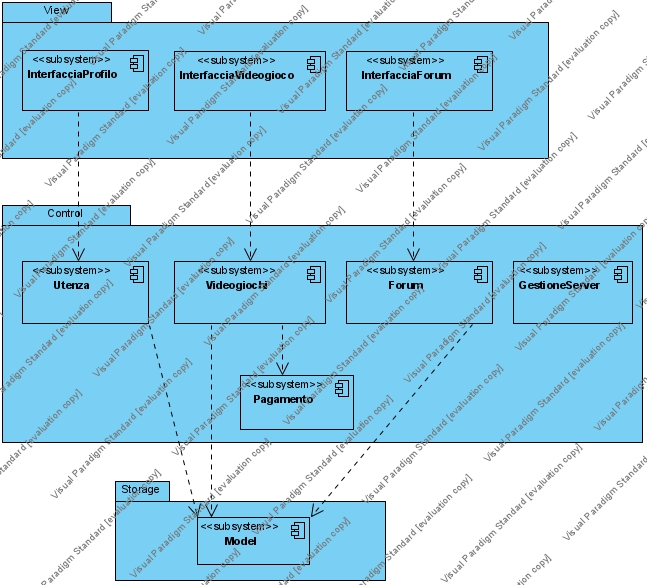
\includegraphics[width=\textwidth,height=\textheight,keepaspectratio]{Figure/SubsystemDiagram.jpg}
\end{center}
\newpage

\section{Mapping Hardware/Software}
L’architettura della distribuzione del sistema segue il modello client/server, dove il client è rappresentato dal Web browser in esecuzione su una macchina di un determinato utente, il quale permette l’accesso ai servizi forniti dal sistema tramite il protocollo HTTP gestendo la parte di visualizzazione delle interfacce e rendendo possibile effettuare richieste. Il server è rappresentato da una singola macchina accessibile dal Web sul quale il sistema è in esecuzione. L’astrazione della fonte dei dati permette l’esecuzione di un database locale per il deployment iniziale del sistema e per la fase di testing, oltre che a permettere una transizione semplice ad un database eventualmente localizzato su una macchina separata, dovendo solo specificare un indirizzo (ed eventuali credenziali) diverso. Il server sarà in comunicazione con il database relazionale tramite uno strato di astrazione (PDO) basato sul protocollo TCP/IP e sarà anche in comunicazione con un filesystem per la gestione di volumi di dati importanti, rappresentati dagli eseguibili dei videogiochi e dalle immagini. Inoltre, il server sarà in comunicazione con il sistema esterno che gestisce i pagamenti, usando come protocollo HTTP, scegliendo come sistema Stripe, il quale permette di pagare con la maggior parte dei circuiti bancari, offrendo una API semplice da usare. Il sistema stesso sarà basato su Laravel, un popolare framework scritto in PHP per lo sviluppo di applicazioni Web robuste, con una API ben documentata e semplice da usare, con tecniche e pattern come l’Inversion of Control, la Dependency Injection e il testing tramite mockups, assieme ad un particolare plug-in ufficialmente sponsorizzato, Cashier, per astrarre la comunicazione con il sistema Stripe. \\
Le interfacce mostrate sui dispositivi posseduti dagli utenti verranno implementate usando come tecnologia il sistema di templating “blade”, simile alle JSP di Java EE, il quale permette la creazione di una pagina HTML con dati dinamici definiti via codice passati come argomenti al template. \\
Sulla macchina del server, invece, verranno implementati i Controller di Laravel, i quali permettono di ricevere una richiesta (eventualmente dopo averla passata attraverso vari middleware, pattern architetturali che trattano la richiesta trasformando eventualmente i dati contenuti o adoperando controlli sulle precondizioni da applicare per quella specifica richiesta. Tali Controller avranno un compito simile agli oggetti Control individuati in fase di analisi, ovvero di orchestrare i modelli necessari per rispondere al tipo di richiesta effettuata dall’utente, ritornando la giusta risposta che l’utente si aspetta sotto forma di file HTML, creato appunto tramite il sistema di templating precedentemente nominato. \\
Oltre ai Controller, verranno anche implementati dei Model, ovvero delle façade di Laravel che fanno parte dell’object relational mapper incluso in Laravel che permettono l’accesso ai dati persistenti del nostro sistema.
\begin{center}
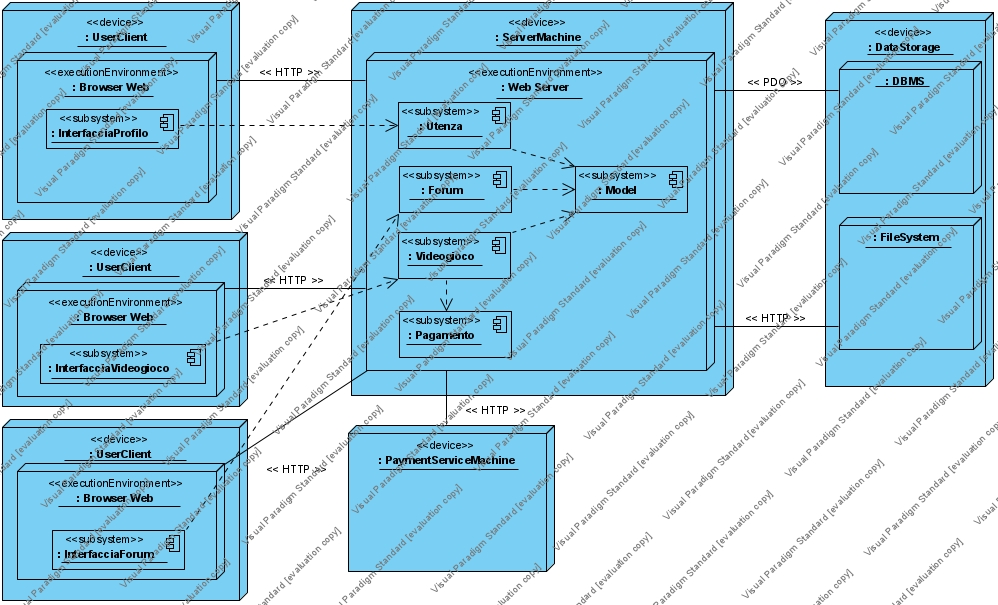
\includegraphics[width=\textwidth,height=\textheight,keepaspectratio]{Figure/Deployment Diagram.jpg}
\end{center}
\newpage
\section{Gestione Dati Persistenti}
Il sistema gestisce i dati persistenti in due modi diversi, a seconda del tipo di dati trattato. Tutti i dati, aventi una determinata struttura ed essendo di dimensioni non importanti, verranno resi persistenti attraverso un database relazionale basato su MySQL, per gestire la concorrenza tra i vari tipi di utenti e i modi in cui richiedono accesso (scrittura o lettura) a tali dati. In particolare, i dati rappresentanti immagini o quello che rappresenta l’eseguibile di un determinato videogioco, scaricabile da un utente previo acquisto se dovuto, verranno anch’essi rappresentati nel database relazionale, ma il dato che verrà effettivamente salvato sarà la locazione sul filesystem del contenuto di tale dato. Per questi tipi di dati non strutturati e voluminosi, quindi, si preferirà una persistenza di tipo semplice, anche perché i casi d’uso principali prevedono un singolo inserimento iniziale e conseguenti letture, negando la necessità di gestire la concorrenza per tali dati.\\
Le classi individuate nel class diagram che verranno rese persistenti saranno:
\begin{itemize}
	\item Utente
	\item Videogioco
	\item VersioneVideogioco
	\item SponsorizzazioneVideogioco
	\item Report
	\item RecensioneVideogioco
	\item ValutazioneRecensione
	\item RichiestaVideogioco
	\item TagVideogioco
	\item Discussione
	\item Commento
\end{itemize}
In particolare, le specializzazioni della classe Utente non riportate come persistenti verranno condensate nella classe Utente, tramite l’aggiunta di un ulteriore attributo il quale rappresenterà il tipo dell’utente (cliente, sviluppatore o amministratore).

\section{Controllo degli Accessi e Sicurezza}
Il sistema deve permettere l’autenticazione degli utenti, in particolare per autorizzarli alle diverse funzionalità in base al loro ruolo. Ciò viene reso possibile offrendo la possibilità di registrarsi e di effettuare il login con le credenziali fornite al momento della registrazione, o eventualmente, nel caso di smarrimento della password, con l’username fornito in fase di registrazione e la password scelta durante il reset. In particolare, si assume l’esistenza a priori di determinati account aventi il ruolo di amministratore.\\
I dati relativi al controllo degli accessi sono memorizzati nel database relazionale, corrispondendo agli attributi della classe Utente “username”, “password” e l’attributo “ruolo” aggiunto per persistere la specializzazione della classe Utente. La password verrà mantenuta rigorosamente nella sua forma hashed, ovvero verrà mantenuto l’hash ottenuto come risultato dell’applicazione della funzione bcrypt, basato sull’algoritmo di hashing Blowfish, usando una chiave privata configurata come variabile di ambiente del sistema. Ciò serve a ridurre i rischi associati ad un eventuale leak dei dati contenuti nel database: per svariati motivi, ciò può succedere, il nostro obiettivo è quello di difendere i dati sensibili dei nostri utenti così da mitigare i danni, in particolare quelli d’immagine, i quali possono essere fatali per un sistema innovativo come GameUp.\\
La fase di login permetterà all’utente di ottenere una sessione, la quale servirà ad autenticarlo per le richieste successive.\\
Le operazioni che ogni attore può effettuare sono dettagliate nella seguente lista di controllo degli accessi, scelta rispetto ad una matrice globale degli accessi per migliorare la leggibilità del codice, avendo dentro una singola classe solo le autorizzazioni relative a quella classe, e anche tenendo conto delle performance, poiché l’implementazione consisterà in una semplice mappa per ogni Controller contenente una operazione associata ad una lista di attori, quindi l’accesso alla lista degli attori avente il permesso per una determinata operazione sarà costante, mentre il controllo relativo alla lista di attori, per vedere se contiene l’attore che sta provando ad effettuare l’operazione, sarà lineare. Tale tempo è considerato trascurabile essendo la lista di attori molto piccola, quindi si adotterà questa struttura principalmente per la leggibilità del codice.\\
Se un utente prova ad accedere ad una operazione senza avere il ruolo richiesto per essa, verrà restituito un errore HTTP 403, basandoci sull’assunzione che l’utente non può fare nulla per poter ottenere l’accesso alla risorsa voluta, poiché il suo ruolo non glielo permette.\\
Nelle tabelle di seguito riportate si assume che l’attore abbia effettuato la procedura di autenticazione per effettuare l’operazione relativa, se non specificato altrimenti.\\
La classe Utente non ha bisogno di un controllo degli accessi basato sul ruolo, poiché tutti gli attori possono effettuare le stesse operazioni rispetto al loro account.\\
La classe Videogioco, invece, offrirà operazioni diverse in base al ruolo dell’attore, come descritto dalla seguente lista:
\begin{center}
	\begin{tabular}{||l | p{16.5em}||} 
	\hline
	\multicolumn{1}{||c|}{\textbf{Operazione}} & \multicolumn{1}{c||}{\textbf{Attori}} \\
	\hline\hline
	ottieniDatiVideogioco & Cliente, Sviluppatore, Amministratore (anche non autenticati) \\ 
	\hline
	infoEssenzialiUltimiVideogiochi & Cliente, Sviluppatore, Amministratore (anche non autenticati) \\ 
	\hline
	ottieniVideogiochiSponsorizzati & Cliente, Sviluppatore, Amministratore (anche non autenticati) \\ 
	\hline
	ottieniVideogiochiPiùScaricati & Cliente, Sviluppatore, Amministratore (anche non autenticati) \\ 
	\hline
	ottieniUltimiGiochiPubblicati & Cliente, Sviluppatore, Amministratore (anche non autenticati) \\ 
	\hline
	ottieniVideogiochiSimili & Cliente, Sviluppatore, Amministratore \\ 
	\hline
	aggiornaDatiVideogioco & Amministratore \\ 
	\hline
	pubblicaVideogioco & Amministratore \\ 
	\hline
	modificaVideogioco & Amministratore \\ 
	\hline
	ottieniLinkDownloadVersione & Cliente, Sviluppatore (se possessori del videogioco), Amministratore \\
	\hline
	nascondi & Amministratore \\
	\hline
	ottieniVideogiochiCompatibili & Cliente, Sviluppatore, Amministratore (anche non autenticati) \\
	\hline
   \end{tabular}
\end{center}

La classe VersioneVideogioco non ha metodi di per se, i dati sono accessibili solo tramite la classe Videogioco e la creazione di una versione deriva dall’aggiornamento o dalla pubblicazione dei dati di un videogioco.\\
La classe SponsorizzazioneVideogioco avrà i seguenti controlli sugli accessi:
\begin{center}
	\begin{tabular}{||l | p{20em}||} 
	\hline
	\multicolumn{1}{||c|}{\textbf{Operazione}} & \multicolumn{1}{c||}{\textbf{Attori}} \\
	\hline\hline
	verificaDisponibilità & Sviluppatore \\ 
	\hline
	creaSponsorizzazione & Sviluppatore (se autore del videogioco) \\
	\hline
   \end{tabular}
\end{center}

\newpage
La classe Report avrà i seguenti controlli sugli accessi:
\begin{center}
	\begin{tabular}{||l | p{23.5em}||} 
	\hline
	\multicolumn{1}{||c|}{\textbf{Operazione}} & \multicolumn{1}{c||}{\textbf{Attori}} \\
	\hline\hline
	risolvi & Amministratore \\ 
	\hline
	creaReport & Sviluppatore (se autore del videogioco) \\
	\hline
	ottieniDettagli & Amministratore \\
	\hline
   \end{tabular}
\end{center}

La classe RecensioniVideogioco avrà i seguenti controlli sugli accessi:
\begin{center}
	\begin{tabular}{||l | p{23em}||} 
	\hline
	\multicolumn{1}{||c|}{\textbf{Operazione}} & \multicolumn{1}{c||}{\textbf{Attori}} \\
	\hline\hline
	salvaRecensione & Cliente, Sviluppatore, Amministratore \\ 
	\hline
   \end{tabular}
\end{center}

La classe ValutazioneRecensione avrà i seguenti controlli sugli accessi:
\begin{center}
	\begin{tabular}{||l | p{23em}||} 
	\hline
	\multicolumn{1}{||c|}{\textbf{Operazione}} & \multicolumn{1}{c||}{\textbf{Attori}} \\
	\hline\hline
	salvaValutazione & Cliente, Sviluppatore, Amministratore \\ 
	\hline
   \end{tabular}
\end{center}

La classe RichiestaVideogioco avrà i seguenti controlli sugli accessi:
\begin{center}
	\begin{tabular}{||l | p{20.5em}||} 
	\hline
	\multicolumn{1}{||c|}{\textbf{Operazione}} & \multicolumn{1}{c||}{\textbf{Attori}} \\
	\hline\hline
	risolvi & Amministratore \\ 
	\hline
	ottieniSintesiRichieste & Amministratore \\
	\hline
	ottieniDettagli & Amministratore \\
	\hline
	nuovaRichiesta & Sviluppatore \\
	\hline
	finalizzaRichiesta & Sviluppatore \\
	\hline
   \end{tabular}
\end{center}

La classe TagVideogioco avrà i seguenti controlli sugli accessi:
\begin{center}
	\begin{tabular}{||l | p{20.5em}||} 
	\hline
	\multicolumn{1}{||c|}{\textbf{Operazione}} & \multicolumn{1}{c||}{\textbf{Attori}} \\
	\hline\hline
	aggiungiSuggerimenti & Cliente, Sviluppatore, Amministratore \\ 
	\hline
	eliminaTags & Cliente, Sviluppatore, Amministratore \\
	\hline
   \end{tabular}
\end{center}

La classe Discussione avrà i seguenti controlli sugli accessi:
\begin{center}
	\begin{tabular}{||l | p{22em}||} 
	\hline
	\multicolumn{1}{||c|}{\textbf{Operazione}} & \multicolumn{1}{c||}{\textbf{Attori}} \\
	\hline\hline
	chiudiDiscussione & Cliente (se autore della discussione), Sviluppatore (se autore del videogioco relativo alla discussione), Amministratore \\ 
	\hline
	poniInRilievo & Sviluppatore (se autore del videogioco relativo alla discussione) \\
	\hline
	creaDiscussione & Cliente (se possiede il videogioco relativo alla discussione), Sviluppatore, Amministratore \\
	\hline
	nascondi & Amministratore \\
	\hline
   \end{tabular}
\end{center}

\newpage
La classe Commento avrà i seguenti controlli sugli accessi:
\begin{center}
	\begin{tabular}{||l | p{22em}||} 
	\hline
	\multicolumn{1}{||c|}{\textbf{Operazione}} & \multicolumn{1}{c||}{\textbf{Attori}} \\
	\hline\hline
	creaCommento & Cliente (se possiede il videogioco relativo alla discussione), Sviluppatore, Amministratore \\ 
	\hline
	nascondi & Amministratore \\
	\hline
   \end{tabular}
\end{center}

\newpage
\section{Controllo del flusso globale del sistema}
Il controllo del flusso globale del sistema è di tipo \emph{thread-driven}, poiché il web-server metterà in una \emph{thread pool} un insieme di thread disponibili e in attesa di gestire le richieste inviate da client multipli. Ogni richiesta verrà gestita da un singolo thread, il quale verrà liberato dopo l’invio della risposta associata al client, potendo così essere riutilizzato per richieste future.

\section{Condizioni Limite}
Per semplificare il più possibile le procedure di startup e shutdown, sfrutteremo il pacchetto Laravel Sail, il quale, basandosi sulla tecnologia dei container Docker, ci permetterà di inizializzare completamente il nostro sistema in un processo isolato tramite un singolo comando, oltre che a poterlo terminare tramite un ulteriore comando. Inoltre, tale pacchetto ci permetterà di avere una serie di container separati, contenenti il nostro database relazionale e la nostra applicazione con tutte le dipendenze necessarie per il framework Laravel. \\
Per la configurazione, l’unico dato necessario durante il primo avvio del sistema è un account amministratore, il quale verrà generato automaticamente durante la creazione del database relazionale con delle credenziali di default (con username uguale ad “admin” e password uguale ad “admin”), con il quale l’amministratore può eseguire l’accesso e cambiare la propria password.
\begin{center}
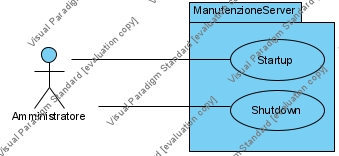
\includegraphics[width=\textwidth,height=\textheight,keepaspectratio]{Figure/ManageServerUseCase.jpg}
\end{center}

L’user task ManutenzioneServer farà parte di un ulteriore sottosistema, GestioneServer.
\subsection{Startup}
\small\begin{tabular}{|| l | p{28em} ||} 
\hline
Nome & Startup\\
\hline
Attori & Amministratore\\
\hline
Condizione d'ingresso & L’amministratore è connesso tramite SSH al server ospitante gli artefatti del sistema ed il sistema non è attualmente in fase di esecuzione.\\
\hline
Flusso degli eventi &
	\begin{tabular}{p{13em}|p{13em}}
	\multicolumn{1}{c|}{\textbf{Utente}} & \multicolumn{1}{c}{\textbf{Sistema}} \\
	\hline
	L’amministratore esegue il comando “./vendor/bin/sail up” dalla cartella root del progetto & \\
	\hline
	& Docker avvia un container contenente l’applicazione Laravel e un container separato come volume contenente l’istanza del database relazionale \\
	\hline
	\end{tabular}
\tabularnewline\hline
Condizione di uscita & Il sistema è completamente inizializzato ed è accessibile tramite un browser Web.\\
\hline
Eccezioni & N/A\\
\hline
Requisiti Speciali & Nel caso il sistema operativo del server sia Windows, è necessaria l’installazione di WSL2.\\
\hline
\end{tabular}

\subsection{Shutdown}
\small\begin{tabular}{|| l | p{28em} ||} 
\hline
Nome & Shutdown\\
\hline
Attori & Amministratore\\
\hline
Condizione d'ingresso & L’amministratore è connesso tramite SSH al server ospitante gli artefatti del sistema ed il sistema è attualmente in fase di esecuzione.\\
\hline
Flusso degli eventi &
	\begin{tabular}{p{13em}|p{13em}}
	\multicolumn{1}{c|}{\textbf{Utente}} & \multicolumn{1}{c}{\textbf{Sistema}} \\
	\hline
	L’amministratore esegue il comando “./vendor/bin/sail down” dalla cartella root del progetto & \\
	\hline
	& Docker ferma tutti i container relativi al sistema \\
	\hline
	\end{tabular}
\tabularnewline\hline
Condizione di uscita & Il sistema non è più in esecuzione e non è più raggiungibile tramite browser Web.\\
\hline
Eccezioni & N/A\\
\hline
Requisiti Speciali & N/A\\
\hline
\end{tabular}

\newpage
\subsection{Fallimenti}
I principali tipi di fallimento che ci si aspetta in fase di esecuzione sono due:
\begin{itemize}
	\item Hardware: Nel caso di un fallimento di tipo hardware sul server ospitante l’applicazione Laravel, non si prevede alcuna strategia di fallback per garantire l’operabilità del sistema. Nel caso il fallimento accada sulla macchina ospitante, verranno effettuati backup settimanali dei dati del database relazionale, mentre per i file eseguibili e per le immagini non verranno adottate strategie di backup.
	\item Software: Nel caso di un problema con l’implementazione del sistema a run-time con una richiesta effettuata da un client, verrà mostrata una pagina generica per comunicare l’avvenuto errore all’utente. La traccia di esecuzione verrà salvata in un file log automaticamente dal framework Laravel, per effettuare il debugging in un secondo momento.
\end{itemize}

\section{Servizi dei Sottosistemi}
\subsection{Utenza}
\begin{center}
	\begin{tabular}{||l | p{22em}||} 
	\hline
	\multicolumn{1}{||c|}{\textbf{Sottosistema}} & \multicolumn{1}{c||}{\textbf{Descrizione}} \\
	\hline\hline
	Utenza & Racchiude tutte le operazioni relative al proprio profilo, alla sua gestione e al suo utilizzo. \\ 
	\hline
   \end{tabular}
\end{center}

\begin{center}
	\begin{tabular}{||l | p{22em}||} 
	\hline
	\multicolumn{1}{||c|}{\textbf{Servizio}} & \multicolumn{1}{c||}{\textbf{Descrizione}} \\
	\hline\hline
	login & Consente ad un utente di autenticarsi al sistema tramite l’username e la password relative al suo account salvato nella piattaforma \\ 
	\hline
	logout & Consente ad un utente di invalidare la propria sessione autenticata \\
	\hline
	registrazione & Consente ad un visitatore di creare un account per potersi autenticare ed effettuare operazioni sensibili \\
	\hline
	tentaRecuperoPassword & Permette ad un utente di iniziare la procedura di recupero password, ottenendo per email un link per finalizzarla \\
	\hline
	resetPassword & Permette ad un utente di finalizzare la procedura di recupero password, effettuando il reset di essa \\
	\hline
	visualizzaProfilo & Permette ad un utente di ottenere i dati associati al proprio profilo, indicati al momento di registrazione o aggiornati in seguito a tale momento \\
	\hline
	modificaProfilo & Permette ad un utente di avviare la procedura di modifica dei dati associati al proprio profilo \\
	\hline
	modificaDatiProfilo & Permette ad un utente di finalizzare la procedura di modifica dei dati associati al proprio profilo \\
	\hline
   \end{tabular}
\end{center}

\subsection{Videogioco}
\begin{center}
	\begin{tabular}{||l | p{22em}||} 
	\hline
	\multicolumn{1}{||c|}{\textbf{Sottosistema}} & \multicolumn{1}{c||}{\textbf{Descrizione}} \\
	\hline\hline
	Videogioco & Racchiude tutte le operazioni relative ai videogiochi della piattaforma, per la creazione e la gestione di essi \\ 
	\hline
   \end{tabular}
\end{center}

\begin{center}
	\begin{tabular}{||l | p{20em}||} 
	\hline
	\multicolumn{1}{||c|}{\textbf{Servizio}} & \multicolumn{1}{c||}{\textbf{Descrizione}} \\
	\hline\hline
	ottieniDatiVideogioco & Permette ad un utente di ottenere le informazioni di dettaglio di un particolare videogioco \\ 
	\hline
	getListaVideogiochi & Permette ad un utente di ottenere una lista di videogiochi paginata, dove per ogni videogioco vengono riportate le informazioni ritenute essenziali in fase di analisi \\
	\hline
	applicaCriteri & Permette di ottenere una lista filtrata di videogiochi paginata, con le stesse informazioni di getListaVideogiochi \\
	\hline
	ottieniVideogiochiSponsorizzati & Permette di ottenere una lista dei videogiochi classificati come sponsorizzati nella data passata come parametro (normalmente la data odierna) \\
	\hline
	ottieniVideogiochiPiùScaricati & Permette di ottenere una lista dei videogiochi più scaricati della piattaforma \\
	\hline
	ottieniUltimiGiochiPubblicati & Permette di ottenere una lista ordinata di videogiochi, in ordine da quello pubblicato più recentemente a quello meno \\
	\hline
	ottieniVideogiochiSimili & Permette di ottenere una lista ordinata di videogiochi, filtrati secondo una analisi di compatibilità con il profilo passato come argomento analizzando le tag dei giochi acquistati precedentemente dall’utente \\
	\hline
	avviaModifica & Permette di avviare la procedura di modifica diretta dei dettagli di un videogioco \\
	\hline
	aggiornaDatiVideogioco & Permette di aggiornare i dati di un videogioco immediatamente \\
	\hline
	ottieniSintesiRichieste & Permette di ottenere una lista di richieste, con i dati ritenuti essenziali in fase di analisi, di pubblicazione e modifica di un videogioco \\
	\hline
	ottieniDettagliRichiesta & Permette di ottenere i dati relativi alla richiesta specificata \\
	\hline
	risolvi & Permettere di risolvere una determinata richiesta \\
	\hline
	modificaVideogioco & Permette di avviare la procedura di creazione di una richiesta di modifica di un videogioco \\
	\hline
\end{tabular}
\end{center}

\begin{center}
	\begin{tabular}{||l | p{20em}||} 
	\hline
	\multicolumn{1}{||c|}{\textbf{Servizio}} & \multicolumn{1}{c||}{\textbf{Descrizione}} \\
	\hline\hline
	richiediPubblicazione & Permette la creazione di una richiesta di pubblicazione di un videogioco \\
	\hline
	finalizzaRichiesta & Permette la finalizzazione di una richiesta di pubblicazione, specificando l’eseguibile della prima versione da caricare del videogioco \\
	\hline
	iniziaSponsorizzazione & Permette di iniziare la procedura di sponsorizzazione di un videogioco \\
	\hline
	selezionaSettimana & Permette di verificare la disponibilità di una settimana, per la sponsorizzazione di un videogioco \\
	\hline
	procediPagamento & Permette la creazione di una sponsorizzazione attraverso il pagamento della somma dovuta \\
	\hline
	acquistaVideogioco & Permette l’aggiunta alla propria libreria di un determinato videogioco, previo pagamento se dovuto \\
	\hline
	downloadVideogioco & Permette il download di una determinata versione di un videogioco \\
	\hline
	avviaProceduraSuggerimentoTags & Permette di avviare la procedura per la gestione dei suggerimenti delle tags di un determinato videogioco \\
	\hline
	seleziona & Permette di selezionare una determinata tag per poterla suggerire \\
	\hline
	consiglia & Permette di suggerire effettivamente una tag per un videogioco \\
	\hline
	rimuoviSuggerimento & Permette di iniziare la procedura di rimozione di un suggerimento tag per un videogioco \\
	\hline
	confermaRimozione & Permette di rimuovere effettivamente una tag \\
	\hline
	valutaRecensione & Permette all’utente di valutare positivamente o negativamente una recensione \\
	\hline
	valutaVideogioco & Permette all’utente di lasciare una propria recensione ad un videogioco acquistato \\
	\hline
   \end{tabular}
\end{center}

\newpage
\subsection{Forum}
\begin{center}
	\begin{tabular}{||l | p{22em}||} 
	\hline
	\multicolumn{1}{||c|}{\textbf{Sottosistema}} & \multicolumn{1}{c||}{\textbf{Descrizione}} \\
	\hline\hline
	Forum & Racchiude tutte le operazioni relative agli spazi dedicati alle comunità di ogni singolo videogioco e le operazioni relative ai report di contenuti offensivi \\ 
	\hline
   \end{tabular}
\end{center}

\begin{center}
	\begin{tabular}{||l | p{20em}||} 
	\hline
	\multicolumn{1}{||c|}{\textbf{Servizio}} & \multicolumn{1}{c||}{\textbf{Descrizione}} \\
	\hline\hline
	chiudiDiscussione & Permette la chiusura di una discussione, per renderla di sola lettura \\
	\hline
	creaNuovaDiscussione & Permette di avviare la procedura di creazione di una discussione \\
	\hline
	creaDiscussione & Permette la creazione di una discussione \\
	\hline
	commenta & Permette all’utente di lasciare un commento in una discussione \\
	\hline
	iniziaReport & Permette di avviare la procedura di reporting per contenuti offensivi \\
	\hline
	creaReport & Permette la creazione di un report associato ad un determinato contenuot ritenuto offensivo \\
	\hline
	poniInRilievo & Permette di porre una discussione in rilievo, mostrandola nella griglia delle discussioni di un forum prima delle discussioni non in rilievo \\
	\hline
	nascondi & Permette di nascondere un contenuto, rendendolo non più visualizzabile da utenti non amministratori \\
	\hline
	visualizzaDettagliReport & Permette di ottenere i dati relativi ad un report \\
	\hline
	risolvi & Permette di marcare un report come risolto \\
	\hline
   \end{tabular}
\end{center}

\subsection{Gestione Server}
\begin{center}
	\begin{tabular}{||l | p{22em}||} 
	\hline
	\multicolumn{1}{||c|}{\textbf{Sottosistema}} & \multicolumn{1}{c||}{\textbf{Descrizione}} \\
	\hline\hline
	GestioneServer & Racchiude le operazioni relative alle procedure di startup e shutdown del sistema da parte di un amministratore \\ 
	\hline
   \end{tabular}
\end{center}

\begin{center}
	\begin{tabular}{||l | p{26em}||} 
	\hline
	\multicolumn{1}{||c|}{\textbf{Servizio}} & \multicolumn{1}{c||}{\textbf{Descrizione}} \\
	\hline\hline
	startup & Permette l’inizializzazione del sistema, procedendo alla creazione di servizi ausiliari nel caso si tratti del primo startup \\
	\hline
	shutdown & Permette di terminare l’esecuzione del sistema in modo sicuro, senza perdite di dati \\
	\hline
   \end{tabular}
\end{center}

\subsection{Pagamento}
\begin{center}
	\begin{tabular}{||l | p{22em}||} 
	\hline
	\multicolumn{1}{||c|}{\textbf{Sottosistema}} & \multicolumn{1}{c||}{\textbf{Descrizione}} \\
	\hline\hline
	Pagamento & Rappresenta il sistema esterno ausiliario atto alla gestione dei pagamenti per videogiochi e sponsorizzazioni \\ 
	\hline
   \end{tabular}
\end{center}

\begin{center}
	\begin{tabular}{||l | p{24em}||} 
	\hline
	\multicolumn{1}{||c|}{\textbf{Servizio}} & \multicolumn{1}{c||}{\textbf{Descrizione}} \\
	\hline\hline
	avviaPagamento & Permette di pagare la somma dovuta per l’acquisto di un videogioco \\
	\hline
	procediPagamento & Permette di pagare la somma dovuta per la sponsorizzazione di un videogioco \\
	\hline
   \end{tabular}
\end{center}

%%%%%%%%%%%%%%%%%%%%%%%%%%%%
\end{document}
